\documentclass[letter,10pt]{article}
\usepackage[utf8]{inputenc}
\usepackage{graphicx}
\usepackage{natbib}
\usepackage{hyperref}
\usepackage{courier}
\usepackage[margin=0.75in]{geometry}
\usepackage[table,svgnames]{xcolor}
\usepackage{multirow}
\usepackage{tabu}
\usepackage{float} \usepackage{listings}
\usepackage{xspace} \bibliographystyle{unsrtnat}
\usepackage[toc,page]{appendix}
\definecolor{HeaderColor}{rgb}{0.8, 0.8, 0.95}
\setlength{\parindent}{0pt}
\setlength{\parskip}{6pt}

\usepackage[T1]{fontenc}
\usepackage[utf8]{inputenc}
\usepackage{authblk}

\author[1,2]{Dimitri Yatsenko\thanks{dvyatsen@bcm.edu}}
\author[1,2]{Edgar Y. Walker}
\author[1,2]{Andreas S. Tolias}
\affil[1]{Department of Neuroscience, Baylor College of Medicine, Houston, Texas, USA}
\affil[2]{Vathes LLC, Houston, Texas, USA}

\renewcommand\Authands{ and }
\newcommand{\datajoint}{DataJoint\xspace}
\date{\today\\Revision 0.1}


\graphicspath{{./figures/}}

\lstset{
    backgroundcolor=\color{AliceBlue},
    tabsize=4,
    basicstyle=\ttfamily\small,
    breaklines=true
    aboveskip={0.5\baselineskip},
    columns=fixed,
    frame=none,
    captionpos=b,
    showstringspaces=false,
    extendedchars=false,
    breaklines=true,
    numbers=none,
    showtabs=false,
    showspaces=false,
    showstringspaces=false,
    framextopmargin=50pt,
    xleftmargin=2pt,
    framexleftmargin=2pt,
    identifierstyle=\color{Black},
    keywordstyle=\bfseries\color{DarkSlateBlue},
    commentstyle=\color{Sienna}\itshape\small,
    stringstyle=\color{Indigo},
    numberstyle=\tiny\color{DarkGray}}

\lstdefinelanguage[]{SSQL}[]{SQL}{
  morecomment=[l][\color{Sienna}\itshape\small]{\#},
  morekeywords={COMMENT, REFERENCES, unsigned}}

\lstdefinelanguage{dj}{
  keywords={int, smallint, char, varchar, enum, unsigned, date, year, decimal, insert, delete, update},
  keywordstyle=\color{blue},
  keywords=[2]{boolean, string, number, objectid},
  keywordstyle=[2]\color{green}\bfseries,
  identifierstyle=\color{Black},
  sensitive=true,
  morecomment=[l][\color{Teal}\bfseries]{::},
  morecomment=[l][\color{Sienna}\itshape\small]{\#},
  stringstyle=\color{Indigo},
  morestring=[b]',
  morestring=[b]"
}

\newfloat{lstfloat}{htbp}{lop}
%\floatname{lstfloat}{Listing}

\title{\datajoint: A Simpler Relational Data Model}

\begin{document}

\maketitle
\begin{abstract}
Proposed here is a simplified and conceptually refined relational data model named \datajoint. 
The model includes a language for schema definition, a language for data queries, and diagramming notation for visualizing entities and relationships among them.  
The model adheres to the principle of \emph{entity normalization}, which requires that all data --- both stored and derived --- must be represented as well-formed entity sets.
\datajoint's data query language is an algebra on entity sets with five operators that provide matching capabilities to those of other relational query languages with greater clarity due to entity normalization. 
Practical implementations of \datajoint in MATLAB and Python have been adopted in several neuroscience labs for fluent interaction with scientific data pipelines.
\end{abstract}
\tableofcontents 

\twocolumn

\section{Core Concepts}
\subsection{The Relational Data Model}
The relational data model \citep{codd_relational_1970} provides the most rigorous approach to structured data storage \emph{and} the most precise approach to querying data.  
The relational data model is defined by the principles of data representation, domain constraints, uniqueness constraints, referential constraints, and declarative queries summarised in Table \ref{tab:core}.

\tabulinesep=6pt
\begin{table*}[ht]
\begin{tabu}{|X|}
\hline
{\bf Data representation.} Data are represented and manipulated in the form of \emph{relations}. 
A relation is a \emph{set} (\emph{i.e.}\ an unordered collection) of \emph{tuples} of values for each of the respective named \emph{attributes} of the relation.
\emph{Base relations} represent stored data while \emph{derived relations} are formed from base relations as a result of data queries.
A collection of base relations with their attributes, domain constraints, uniqueness constraints, and referential constraints is called a \emph{schema}.

\\
{\bf Domain constraints.} Attribute values are drawn from corresponding attribute \emph{domains}, \emph{i.e.}\ predefined sets of values.
Attribute domains may not include other relations, ensuring that the relational model is essentially flat with no nesting data structures.

\\
{\bf Uniqueness constraints.} Tuples within relations are addressed by values of their attributes.
To identify and relate data elements, \emph{uniqueness constraints} on a subset of attributes may be imposed so that no two tuples can have the same values of these attributes.  The set of attributes with a uniqueness constraints are referred to as a \emph{key}. One in a relation key may be designated as the \emph{primary key} for the relation to serve for referencing elements in a relation.

\\
{\bf Referential constraints.} Associations among data are established by means of \emph{referential constraints} in the form of \emph{foreign keys}. 
Referential constraints prohibit tuples in one relation unless the referenced relation already contains tuples with matching values of corresponding attributes. 

\\
{\bf Declarative queries.} \emph{Queries} produce derived relations from base relations and retrieve the result.  
\emph{Query expressions} provide declarative specifications for retrieved data rather than procedural specifications typical of other data models. 
Formal languages for query expressions include \emph{relational algebra} and \emph{relational calculus}.  
\\
\hline
\end{tabu}
\caption{Core principles of the relational data model.}
\label{tab:core}
\end{table*}

Popular implementations of the relational data model rely on the Structured Query Language (SQL).
SQL comprises distinct sublanguages for schema definition, data manipulation, and data queries.
SQL so thoroughly dominates in the space of relational databases that, in casual discourse, SQL and the relational data model have become conflated. 

\datajoint is a clean, consistent, and conceptually refined implementation of the relational data model adhering faithfully to its core principles.
Its introduction is motivated by the need for expressive and rigorous  constructs for database programming in scientific computing.

\datajoint comprises 
\begin{itemize}
\item a \emph{schema definition language} (Sec.\ \ref{sec:def1} and \ref{sec:def2})
\item a \emph{data manipulation language} (Sec.\ \ref{sec:manip})
\item a \emph{data query language} (Sec.\ \ref{sec:query})
\item diagramming notation for visualizing relationships between modeled entities (Sec.\ \ref{sec:diag}).
\end{itemize}

Relations are often visualized as \emph{tables} with attributes corresponding to \emph{columns} and tuples corresponding to \emph{rows}.  
In particular, SQL uses these terms rather than those of the formal relational model.  
Table \ref{tab:terms} correlates equivalent terms used in different variants of the relational data model.

\tabulinesep=6pt
\begin{table*}[ht]
   \rowcolors{1}{white}{gray!20}
   \begin{tabu}{|X[1,c,p]| X[1,c]| X[1,c]| X[1,c]|}
   \hline
   \rowcolor{HeaderColor}
   {\bf Relational} & {\bf ERM} & {\bf SQL} & {\bf \datajoint}  \\
   \cellcolor{white} & entity set & \cellcolor{white} & \cellcolor{white} \\
   \multirow{-2}{*}{relation}  & relationship set  & \multirow{-2}{*}{table}  &  \multirow{-2}{*}{entity set} \\
   tuple       & entity           & row    & entity \\
   domain      & value set        & data type & data type \\
   attribute   & attribute        & column {\em or} field    & attribute \\
   attribute value & attribute value  & field value & attribute value \\
   primary key & primary key & primary key & primary key \\
   foreign key & foreign key & foreign key & foreign key {\em or} dependency \\
   schema      & schema      &  schema  &  schema \\
   relational expression \par {\em or} derived relation &  data query & {\tt SELECT} statement & query expression \\
   \hline
   \end{tabu}
\caption{Corresponding terms used in variants of relational models.}
\label{tab:terms}
\end{table*}

\subsection{Conceptual Ambiguity}
The relational model is abstract and semantically unconstrained, providing few guidelines for translating problems into database schemas or for forming valid queries. 
Learning to design and query databases for practical problems requires \emph{conceptual clarification}: developing intuition and techniques for mapping real-world rules onto the concepts of the relational data model from Table \ref{tab:core}.

A set of formal rules known as \emph{normal forms} have been devised to test whether a particular schema meets basic quality requirements that preclude redundancies in data storage and avoid anomalies in data manipulations \citep{kent-1983-simple}.  
Relying on the mathematical concept of {\em functional dependencies} among the attributes, normal forms remain abstract and provide no conceptual clarification. 
When a schema does not meet the normal forms, it is considered \emph{unnormalized}; whereas redesigning schemas to meet these tests is called \emph{normalization}.
SQL does not provide mechanisms for enforcing or diagnosing normalization in its data definition language. 
It takes considerable training to educate database programmers about the design of normalized schemas in the general case. 

For data queries, the relational data model provides few constraints as to what constitutes a valid or meaningful query, allowing unlimited freedom to compare, match, and combine attributes of relations regardless of their semantic compatibility.

New practitioners enter the field of database programming with their diverse backgrounds and mindsets, conceiving of database tables as spreadsheets with arbitrary semantics of rows and columns.  
Only with experience in more sophisticated designs, do they develop, mostly implicitly, various semantic mappings of real-world information motifs and database design pattens.

The overall lack of semantic constraints in the relational data model and SQL in particular leaves great freedom to experienced developers with honed conceptual skills. But it also allows for a great diversity of incompatible approaches to schema design and data queries and lengthens the path from mediocrity to proficiency.

\subsection{Entity-Relationship Model}
The most successful effort to clarify the relational data model began with the Entity-Relationship Model (ERM) \citep{chen_entity_1976}.  
The ERM provides 
\begin{enumerate}
\item a method for problem analysis for schema design 
\item diagramming notation for schema design 
\item constraints for meaningful queries
\end{enumerate}

The central concept in ERM is that of an {\em entity set}: an unordered collection of identifiable items (entities) in the modeled world that share the same set of attributes, are distinguished from each other by the same \emph{primary key}, and can participate in the same types of relationships with other entity sets. 
In ERM, all base relations are either entity sets or \emph{relationship sets} between entity sets; these terms effectively subsume the term \emph{relation} (Table \ref{tab:terms}).

ERM diagramming notation depicts entity sets and relationship sets, turning ERM into an effective tool for \emph{conceptual modeling} and communication between database designers, customers, and managers.
For example, Panel {\sf A} in Figure \ref{fig:erm-notation} depicts a simple entity-relationship diagram for a university student database with two entity sets, {\tt Student} and {\tt Department} and the relationship {\tt majors in} between them.

\begin{figure}
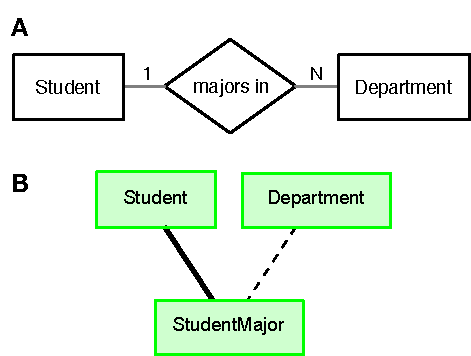
\includegraphics{major-erd.pdf}
\caption{
{\sf A:} The entity-relationship diagram of a database schema model university departments, students,  and their major department using ERM diagramming notation.
{\sf B:} A similar schema in the \datajoint model and diagrammed in \datajoint notation.}
\label{fig:erm-notation}
\end{figure}


A \emph{relationship set} is a collection of associations linking entities from two or more entity sets and sharing the same set of attributes. 
These associations take the form of referential constraints (foreign keys) between relationships sets and entity sets.
Although the ERM is mostly known for its approach to schema design, it also prescribes methods to form valid data queries: Queries must rely on foreign keys to match entities through the relationships in which they participate. 

ERM was proposed as a complete data model in its own right but its conceptual refinements were never translated into a practical programming language and, today, ERM is best known as a diagramming technique only.  
Formal courses in database programming prescribe a two-phased approach to database design: \emph{conceptual modeling} using a diagramming tool such as ERM followed by translation or (\emph{logical  design}) into a relational database schema and SQL \citep{elmasri-2015-fundamentals, coronel-2016-database}. 
Trained database designers mentally internalize ERM principles in their approach to schema design and queries.
They often explicitly or mentally categorize tables as either ``entity tables'' or ``relationship tables'' even though SQL makes no such distinction. 
Such partitioning of entities and their relationships onto distinct relations in a database schema yields designs that are naturally normalized, \emph{i.e.}\ they pass the criteria of normal forms. 
ERM-based designs tend to naturally produce database schemas that already  meet rules of database normalization from formal relational database theory so that practicing database developers rarely need to recall the definitions of normal forms from their formal academic training.
When using the ERM approach, the problem of database normalization is translated into a more relatable problem of correctly distinguishing entities in the modeled world.  
We will refer to this approach to database normalization as \emph{entity normalization} described in depth in section \ref{sec:norm}.


Could a programming language tailored to ERM be made clearer and more expressive, making it easier to learn and to use than the more general relational model and SQL? 

For example, in the general relational data model, a foreign key may reference an arbitrary subset of attributes. In the ERM, the foreign key always references the primary key of the referenced entity set with an equivalent subset of attributes in the referencing relationship set.  Therefore, an ERM-specific schema definition language could simplify the definition and use of foreign keys.

Consider the following section of SQL table definition code defining a foreign key to the {\tt Course} table whose primary key comprises attributes ({\tt dept}, {\tt course}):
\begin{lstlisting}[language=SSQL]
dept char(6) NOT NULL COMMENT 
  "abbreviated department name, e.g. BIOL",
course int unsigned NOT NULL COMMENT 
  "course number, e.g. 1010",
FOREIGN KEY (dept, course) 
  REFERENCES Course(dept, course)
\end{lstlisting}
In an ERM-tailored language, the equivalent foreign key definition could become simply
\begin{lstlisting}[language=dj]
-> Course
\end{lstlisting}
if the referencing attribute names are the same as the referenced names.

The simplified definition combines two jobs into a single step:  add the referencing attributes to the table definition (if not already added) and create the foreign key constraints.  These definition are not only more terse but are less error-prone since changes in the definitions of the referenced table would automatically and correctly propagate to the referencing table. 

This syntax simplification would serve well in the majority (perhaps 99\%) of common uses of foreign keys since they typically follow ERM conventions. What should be done for the more esoteric uses of the relational model that define foreign keys referencing non-primary key attributes of the referenced table (For example, fifth normal form)?  Perhaps we could add special syntax to accommodate such rare cases. Perhaps the preferred solution is to simply accept the loss of representational power for the arguably more valuable gain in conceptual clarity. 

Since ERM constrains schema definitions, it reduces the representational power of the general relational data model and skirts around some of its more esoteric capabilities. 
For example, ERM is incapable of representing multiple functional dependencies between overlapping sets of attributes whereas the broader relational theory can accomplish such feats through use of referential constraints prohibited in ERM {\em cf.\ fifth normal form}.
Giving up some representational power was deemed a fair tradeoff for increased conceptual clarity.  The gain in conceptual clarity for practical database design processes was thought to outweigh the loss of capabilities.

\subsection{\datajoint Model}
\datajoint embodies a single coherent data model that is sufficient for clear conceptual modeling, efficient schema design, and precise and flexible data queries. 
Similar to ERM, \datajoint is a conceptual clarification of the relational data model.  
But it differs from ERM in several key ways. 
First, in \datajoint, no distinction is made between entity sets and relationship sets.  All data are modeled as entity sets.
Entity sets do participate in \emph{dependencies} on one another in the form of referential constraints.  The term \emph{relationship} is used more generally to describe various  effects of dependencies between entity sets.

In ERM, for example, Marriage might be modeled as a binary relationship set between entity set of type Person.  In \datajoint, Marriage is modeled as an entity set with two dependencies referencing Person. 

Relations and entity sets are often visualized in the form of \emph{tables}. 
Therefore, in \datajoint the terms \emph{relation}, \emph{entity set}, and \emph{table} can be used interchangeably even though this equivalence does not generally hold in other data models. 
Individual elements of an entity set may be called \emph{entity instances}, \emph{tuples}, or \emph{rows}.
The attributes of an entity set may also be called \emph{columns} or \emph{fields}. (See Table \ref{tab:terms}).

In \datajoint, referential constraints are often called \emph{dependencies} or \emph{foreign keys}.  
The composition of foreign keys between entity sets results in a rich variety of relationships. 
To expressively depict this variety of dependencies, \datajoint introduces its own diagramming notation.

\subsection{Entity normalization}\label{sec:norm}
By \emph{entity normalization} we denote the requirement that all data exist in the form of relations that meet the criteria of well-formed entity sets.

A well-formed entity set is a relation that meets the following criteria:
\begin{enumerate}
\item All elements of the relation belong to the same well-defined and readily identified entity type from the model world.
\item All attributes of the relation are applicable directly to each of its elements, although some attribute values may be missing (set to null).  
\item All elements of the relation must be distinguishable form each other by the same \emph{primary key}.
\item Primary key attribute values cannot be missing (set to null).
\item All elements of the relation participate in the same types of relationships with other entity sets.
\end{enumerate}

Adherence to entity integrity is the common thread unifying \datajoint's data definition language, data manipulation language, and data query language. 
\datajoint respects entity normalization in both base relations and derived relations resulting from query operations (Sec.\ \ref{sec:query}.  
In schema design, entity normalizations serves as the guiding principle for efficient and sensible design.
For queries, \datajoint's relational operators are designed so that each intermediate result constitutes a valid entity set meeting all the above criteria.

Entity normalization bears parallels with two concepts from conventional relational database theory: \emph{normal forms} and the \emph{entity integrity constraint}.
Decomposition  of data into entity sets that meet Criteria 1--5 ensure that the schema meets the criteria defined by the Boyce-Codd normal form.

In established relational database theory, the \emph{entity integrity constraint} refers to the requirement that base relations in a schema  must have an explicitly defined primary key and that values of the primary key attributes cannot be missing (set to null).  
This is a much narrowed definition of entity integrity.

\section{Schema Definition}\label{sec:def1}
\subsection{Entity definition syntax}
\datajoint's  \emph{schema definition language} allows defining entity sets for stored data or \emph{base entity sets} and dependencies between them. 
Base entity sets are identified by unique names within their schema. 

A university database is a popular example for demonstrating database design and we will design a simple database to illustrate basic concepts. 
Listing \ref{lst:uni1} defines three base entity sets {\tt Student}, {\tt Department}, and {\tt StudentMajor}.

\begin{lstfloat*}
\begin{lstlisting}[language=dj,caption={University database schema definition (Part 1).},label={lst:uni1}]
::Student     
student_id : int unsigned   # university-wide ID number 
---
first_name      : varchar(40)
last_name       : varchar(40)
sex             : enum('F', 'M', 'U')
date_of_birth   : date
home_address    : varchar(200) # street address
home_city       : varchar(30) 
home_state      : char(2)  # two-letter abrreviation
home_zipcode    : char(10)
home_phone      : varchar(14) 

::Department 
dept : char(6)   # abbreviated department name, e.g. BIOL
---
dept_name    : varchar(200)  # full department name
dept_address : varchar(200)  # mailing address
dept_phone   : varchar(14)  

::StudentMajor
-> Student
---
-> Department
declare_date :  date  # when student declared her major  
\end{lstlisting}
\end{lstfloat*}

Each entity set begins with the line specifying the entity name as 
\begin{lstlisting}[language=dj]
::EntityName 
\end{lstlisting}

By convention, the name of the entire entity set describes an individual entity rather than the entire entity set.  
Thus the entity set {\tt Student} contains all students from our university. 

\subsubsection{Attributes and their datatypes}
The remaining lines of an entity definition define entity attributes in the form
\begin{lstlisting}[language=dj]
attribute_name : datatype   # comment
\end{lstlisting}
The comment is optional.

A variety of datatypes may be used.  In our examples, we will use the following datatypes familiar from SQL.
\begin{itemize}
\item \lstinline$int$ -- 32-bit signed integer 
\item \lstinline$int unsigned$ -- 32-bit unsigned integer
\item \lstinline$decimal(n,m)$ -- decimal number with {\tt n} total digits and {\tt m} fractional digits
\item \lstinline$char(n)$, \lstinline$varchar(n)$ -- a string of up to {\tt n} characters
\item \lstinline$date$ -- calendar date
\item \lstinline$year$ -- calendar year 
\item \lstinline$enum('one','two','three')$ -- element from the enumerated set of values
\end{itemize}

\begin{lstfloat*}
\begin{lstlisting}[language=dj,caption={University database schema definition (Part 2).}, label={lst:uni2}]
::Course     
-> Department
course  : int unsigned   # course number, e.g. 1010
---
course_name :  varchar(200)  # e.g. "Neurobiology of Sensation and Movement."
credits     :  decimal(3,1)  # number of credits earned by completing the course

::Term
term_year : year 
term      : enum('Spring', 'Summer', 'Fall')

::Section 
-> Course
-> Term 
section : char(1)
---
auditorium   :  varchar(12)

::CurrentTerm
---
-> Term

::Enroll
-> Section
-> Student 

::LetterGrade
grade : char(2)
---
points : decimal(3,2)

::Grade 
-> Enroll
---
-> LetterGrade

\end{lstlisting}
\end{lstfloat*}

\begin{figure}
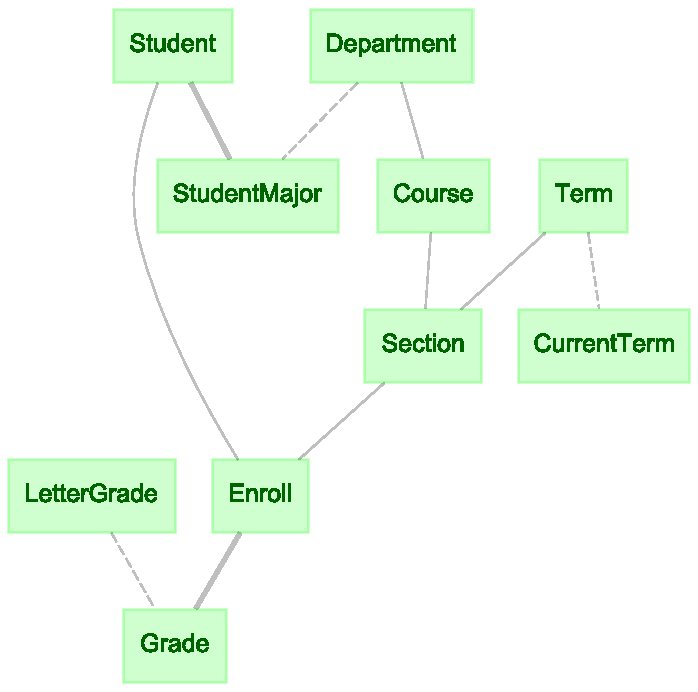
\includegraphics[width=\columnwidth]{uni_erd.pdf}
\caption{The schema diagram of the university database.}
\label{fig:erd}
\end{figure}


\subsection{Primary key}
A major ingredient of \emph{data integrity} is \emph{entity integrity}: identifiability and uniqueness of entity representations in the database. 
{Primary keys} are the principal tool for communicating and enforcing entity integrity. 
Any entity set must have a primary key: a set of attributes that, jointly, distinguish elements of the relation from each other.
No two elements of the same entity set can share the same value of the primary key or, in other words, the same combination of values of the primary attributes.

In each table declaration (e.g.\ Listings \ref{lst:uni1} and \ref{lst:uni2}), the dividing line \lstinline$---$ separates the \emph{primary key} attributes above from other attributes below.  
Each entity set must have a primary key although it may comprise multiple attributes. 
For brevity, we refer to the attributes in the primary key as \emph{primary attributes} and all others as \emph{secondary attributes}.

For example, the primary key of entity set \lstinline$Student$ (Listing \ref{lst:uni1}) contains one attribute \lstinline$student_id$.  
No two elements in \lstinline$Student$ can share the same value of \lstinline$student_id$. 
Consequently, any element can be uniquely identified by \lstinline$student_id$ alone. 

The primary key of entity set \lstinline$Term$ (Listing \ref{lst:uni2}) contains two attributes: \lstinline$term_year$ and \lstinline$term$.
This means that a pair of elements of \lstinline$Term$ can be in the same \lstinline$term_year$ or in the same \lstinline$term$ but cannot be together in both. 

If the primary key of a particular entity set contains zero attributes, it cannot distinguish any two elements within the set.  
Consequently, an entity set with an empty primary key can contain only one element at most.
This makes sense for entity set \lstinline$CurrentTerm$ in Listing \ref{lst:uni2}, which contains the value of the academic term currently in session; and only one session can be current at any time.

\subsubsection{Phantom attribute $\omega$}\label{sec:phantom}
In explaining the \datajoint data model, we find helpful to introduce the concept of the phantom attribute $\omega$ that is always present in the primary key of any entity set.  
The domain of $\omega$ contains only one element, \lstinline$"1"$, which is also the default value for $\omega$.
The phantom attribute is entirely contrived since it carries no information: all elements of any entity set would always have the same value for this attribute.
However, the phantom attribute may help in conceptual understanding and interpretation of the model.
For example, one may think of the empty primary key of \lstinline$CurrentTerm$ as rather a primary key comprising only the phantom attribute $\omega$, which can only take on one value.
 
\subsubsection{No surrogate keys}
In established database terminology, the term \emph{surrogate key} describes an attribute that is internally assigned by the database system to uniquely identify elements of an entity set. 
Strategies for generating surrogate key values include serial numbers and universally-unique identifiers (randomized sequences of sufficient length to guarantee uniqueness).
\emph{Surrogate} keys are contrasted with \emph{natural} keys, which comprise identifying attributes already associated with the entity set in ``the real world''.

For \datajoint, we dismiss the concept of surrogate keys as logically incongruous in favor of a more consequential distinction.
Namely, the important question to ask about any entity set is:
\begin{quote}
\em
Does the overall process ensure a unique mapping between the primary key values of the entity set and the real entities that it claims to represent?
\end{quote}

If the answer is \emph{yes}, then it matters not whether the primary key values are generated by the database system or come from the ``real world''. 
Indeed, trusted system-generated identifiers tend to leak into the external world, confounding the distinction between ``natural'' and ``surrogate''.
Other entities may be defined to exist entirely within the database system (\emph{e.g.}\ logged events) and for them the ``real word'' and the database system are one and the same.

If the answer to the question above is \emph{no}, then the entity set cannot claim to represent the real entities in question. 
Then the proper course of action must  be to either (a) ensure a unique mapping or (b) change the name and description of the entity set to a more accurate one, for which the answer is \emph{yes}. 

For example, by naming the entity set \lstinline$Student$, I declare that I have ensured a reliable process for a unique mapping between students in the real world and the values of the primary key of \lstinline$Student$.
In this case, I need to ensure that there is a personal verification process that precludes assignment of multiple student IDs to the same student or the same ID to multiple students.
If the university system lacks such mechanisms and only ensures uniqueness of records by a ``surrogate key'', then I do not have the right to name the entity set \lstinline$Student$.
I should name it \lstinline$StudentRegistrationRecord$, for example, without implication of a unique mapping to real students.

In summary, \datajoint does not admit the concept of surrogate keys.  
Instead, it requires reliable unique identification for the elements of well-defined and accurately described entity sets.

\subsection{Dependencies}
Another ingredient of data integrity is \emph{referential integrity}, which in \datajoint is communicated and enforced through \emph{foreign key dependencies} or simply \emph{dependencies}.

A foreign key dependency is declared in a table definition as 
\begin{lstlisting}
-> Ref 
\end{lstlisting}
where \lstinline$Ref$ is another entity set.

For example, entity set \lstinline$StudentMajor$ (Listing \ref{lst:uni1}) declares two dependencies: on \lstinline$Student$ from its primary key and on \lstinline$Department$ as a secondary attribute.

In the simpler use cases shown in Listings \ref{lst:uni1} and \ref{lst:uni2}, the referenced entity sets are base. 
Section \ref{sec:dep} describes more general cases when \lstinline$Ref$ may be derived entity sets.

\subsubsection{Effects of dependencies}\label{sec:effects}
If the new table \lstinline$Dependent$ declares the dependency \lstinline$-> Ref$, then this declaration has the following effects: 
\begin{enumerate}
\item The primary key attributes of \lstinline$Ref$ are added to the definition of \lstinline$Dependent$ skipping those that are already present in the definition.
\item The referential constraint is created prohibiting tuples in \lstinline$Dependent$ without \emph{matching} entries in \lstinline$Ref$.
\item An index is created in \lstinline$Dependent$ for fast search in \lstinline$Dependent$ given primary key values of \lstinline$Ref$.
\end{enumerate}

The referential constraint is enforced by (a) prohibiting inserts into \lstinline$Dependent$ of elements that are missing the matching elements in \lstinline$Ref$ and (b) propagating deletes from \lstinline$Ref$ to \lstinline$Dependent$ of all matching tuples.

\subsubsection{Schema diagrams}\label{sec:diag}
Entire schemas or portions of schemas may be visualized using \datajoint's diagramming notation.  
For example, the schema defined in Listings \ref{lst:uni1} and \ref{lst:uni2} is diagrammed in Figure \ref{fig:erd}. 
Each base entity set (table) becomes a named node in the graph with foreign key dependencies represented as its edges. 

\subsubsection{Primary and secondary dependencies}
When entity set \lstinline$B$ declares a dependency of entity set \lstinline$A$ from its primary key, the primary key attributes of \lstinline$A$ become incorporated in the primary key of \lstinline$B$.  
Dependencies declared from the primary key are called \emph{primary dependencies} and are indicated with solid lines on the schema diagram. 
Dependencies declared from the outside the primary key are called \emph{secondary dependencies} and are indicated with dashed lines in the schema digram.  
In a secondary dependency, the primary attributes of \lstinline$A$ are added as secondary attributes \lstinline$B$. 

Primary dependencies indicates a much closer \emph{defining relationship} between the entities. Whereas secondary dependencies create a merely \emph{referential relationship}.

For example, the entity set \lstinline$StudentMajor$ declares a primary dependency onto \lstinline$Student$ and a secondary dependency onto \lstinline$Department$ (Listing \ref{lst:uni1} and Figure \ref{fig:erd}).

\subsubsection{Acyclicity}
In \datajoint, the graph of dependencies never contains loops or cycles.  
In other words, any dependency diagram is an \emph{acyclic directed graph}.
This constraint may seem unnecessary since the model can be straightforwardly extended to allow cyclic dependencies. 
However, we find that conceptual complications arising from cyclic dependencies are not worth the benefits that they bring and we make the \emph{acyclicity} of dependencies a key property of the \datajoint model.

The acyclicity of dependencies in the model does not mean that the model is not capable of representing cyclic \emph{relationships}. 
However, it does mean that sometimes an extra entity set is necessary to represent cyclic relationships. 

\subsubsection{Semantics of dependencies}\label{sec:semantics}
In \datajoint, dependencies are established between entire entities rather than between attributes of entities.  
When entity set \lstinline$B$ depends on entity set \lstinline$A$ by means of a foreign key constraint, all attributes of their elements are thought to be constructed with respect to all attributes of the referenced elements of \lstinline$A$.

\section{Data manipulation}\label{sec:manip}
The two basic commands for data manipulation are \emph{insert} and \emph{delete} to add or remove new elements (tuples) into base entity sets.

\subsection{Insert}
The \emph{insert} command inserts new elements into an existing base entity set.  
The elements (entities) to be inserted must be fully formed and the entire set is added atomically.
Invalid elements are rejected. 
An element may be invalid if it is incomplete, or if it violates a domain constraint (incorrect value datatype), or if it violates a unique constraint (duplicate value in the primary key), or a referential constraint (no matching entry in a referenced entity set).
When an insert is rejected for any one element, the entire insert set is rejected.

Example:
\begin{lstlisting}[language=dj]
insert Student (student_id, first_name, last_name, sex, date_of_birth, student_address, student_phone):
(1000, 'Rebecca', 'Sanchez', 'F', 1997-09-13, '6604 Gentry Turnpike Suite 513', 'Andreaport', 'MN', '29376', '(250)428-1836'),
(1001, 'Matthew', 'Gonzales', 'M', 1997-05-17, '1432 Jessica Freeway Apt. 545', 'Frazierberg', 'NE', '60485-3810', '(699)755-6306x996')
\end{lstlisting}

\subsection{Delete}\label{sec:delete}
The \emph{delete} command removes a subset of elements from a base entity set and the corresponding dependent subsets from any dependent entity sets, cascading recursively down the chains of dependencies.
Deletes cascade recursively to dependent entities according to the foreign keys constraints so that deleting an entity from one entity set triggers the deletion of all matching entities downstream in the data pipeline.
Individual delete commands are executed atomically, no matter how many elements are deleted and how far downstream they cascade along dependency chains.
To specify the subset of elements to remove, delete relies on restriction operator (Sec.\ \ref{sec:restrict}).

Example: 
\begin{lstlisting}[language=dj]
delete Student & student_id > 500 & student_id <= 1000
\end{lstlisting}

\subsection{Cautious updates}
The \emph{update} operation modifies the values of individual attributes in an entity set.
Although very common in other data models, updates are used sparingly in \datajoint. 
The principal way to change the state of a \datajoint database is to delete and insert subsets of entire entities with all their attribute values already set. 

Updating values in place is a precarious proposition from the point of view of data integrity. 
This has to do with the interpretation of referential constraint.  
When a foreign key from entity set \lstinline$B$ references entity set \lstinline$A$, this means that elements in \lstinline$B$ are generated with respect to the value of the referenced entities in \lstinline$A$ in their entirety.  
Modifying the attributes of entities of \lstinline$A$ will invalidate this assumption.
For example, if entries of \lstinline$Section$ are generated referencing \lstinline$Course$, which are in turn referenced by \lstinline$Enroll$, then changing the name of the course or the number of credit hours in \lstinline$Course$ would fundamentally change the meaning of entries downstream in the pipeline.  
If the name of the course changes in any way, then downstream entries need to be reevaluated in light of the change.
This is particularly critical in computational pipelines where downstream entity sets contain results of computations that are based on values upstream in the pipeline.  

The \datajoint model works under a fundamental data integrity contract: data inserted downstream in the dependency graph rely on the immutability of the upstream data. 
For these reasons, updates are not part of the data manipulation model in \datajoint.

However, in cases when users are confident that an update is safe and appropriate, an update operator may be provided.

For example, the following operation updates the phone number for student ID 1001:
\begin{lstlisting}[language=dj]
update Student & student_id == 1001:
    phone = "(713)555-1040x101"
\end{lstlisting}

\section{Query Expressions}\label{sec:query}

\subsection{Relational operators and expressions}
Query expressions use \emph{relational operators} to combine base entity sets to form new \emph{derived entity sets} for precise data queries.
The result of a data query is a symbolic representation of the derived entity set: when the state of the database changes, so does the result of a query expression.
\datajoint has only six relational operators summarized in Table \ref{tab:operators}.
\datajoint's query expressions are \emph{algebraically closed}:  derived entity sets can be assigned to variables or used in other expressions to formulate ever more exact or complex queries.

\begin{table}[ht]
\rowcolors{1}{gray!20}{white}
\begin{tabu}{|X[1,c,p,0.3cm] X[1,c,1.6cm] X[1,c,p,1.6cm]|}
\hline
\rowcolor{HeaderColor}
{\bf operator} & {\bf notation} & {\bf result} \\
{\bf restrict} (Sec.\ \ref{sec:restrict})  & \lstinline$A \& cond$  & The subset of all elements of \lstinline$A$ that meet condition \lstinline$cond$ \\
{\bf exclude} (Sec.\ \ref{sec:restrict}) & \lstinline$A \\ cond$  & The subset of all elements of \lstinline$A$ except those that meet condition \lstinline$cond$ \\
{\bf join} (Sec.\ \ref{sec:join}) & \lstinline$A * B$ & The combination of matching elements of \lstinline$A$ and \lstinline$B$ \\
{\bf project} (Sec.\ \ref{sec:proj}) & \lstinline$A.proj(...)$ & Select, rename, and calculate attributes for \lstinline$A$ \\
{\bf aggregate} (Sec.\ \ref{sec:aggr}) & \lstinline$A.aggr(B, ...)$ & Calculate new attributes for \lstinline$A$ using aggregation operations on attributes of matching entries in \lstinline$B$ \\
{\bf union} (Sec.\ \ref{sec:union}) & \lstinline$A + B$ & The set of elements that are in either \lstinline$A$ or \lstinline$B$ or both. \\ 
\hline
\end{tabu}
\caption{\datajoint query operators.}
\label{tab:operators}
\end{table}

\subsection{Operational entity normalization}\label{sec:operational}
In \datajoint, the principle of \emph{entity normalization} (Section \ref{sec:norm}) extends to derived entity sets.
Any operator produces a well-defined entity class with a designated primary key. 
We refer to this property of \datajoint expressions as \emph{operational entity normalization}. 
Operational entity normalization sets apart from other relational query languages, which limit the formal application of concepts of normalization and entity integrity to base entity sets.

\subsection{Matching attributes}\label{sec:match}
The binary operators in query expressions (join, restriction,  exclusions, and aggregation) require matching attributes in the two arguments for the equality comparison underlying the operation. 
The choice of the attributes to match define the semantics of the operation. 
In other relational querly languages, the matching attributes must be specified explicitly in each operator, forcing developers to examine the semantics of the attributes and to write unwieldly queries.
One shortcut to specifying matching attributes in relational algebra and SQL is used in the \emph{natural join}, where attributes are considered matching when they share the same name, based on the assumption that attributes with the same name are related semantically to correctly restrict the result.
However, natural joins lead to frequent mistakes in cases when unrelated attributes happen to share the same names.

\datajoint has a single uniform method to define the semantic of binary operators through matching attributes.  
In this method, the matching attributes are those that share the same names in both operands of the binary operator \emph{and} trace their origin through foreign keys to the same original primary attribute of the same base entity set.
This approach ensures that the matching operators have the same meaning. 

For example, the entity sets \lstinline$StudentMajor$ and \lstinline$Enroll$ (Listings \ref{lst:uni1} and \ref{lst:uni2} Figure \ref{fig:erd}) have matching attributes \lstinline$student_id$ and \lstinline$dept$, which they acquire through a series of dependencies from the primary key of \lstinline$Student$ and \lstinline$Department$, respectively.  

Then, in the binary operators 
\begin{itemize}
\item join \lstinline$StudentMajor * Enroll$ 
\item restriction \lstinline$StudentMajor & Enroll$ 
\item exclusion \lstinline$StudentMajor \ Enroll$ 
\item aggregation \lstinline$StudentMajor.aggr(Enroll, n=count())$ 
\end{itemize}
 the equality of the values in these attributes from the two inputs determines the output of the operator.

\datajoint's approach is more semantically refined than previously defined matching schemes since it ensures the semantic equivalence of the matching attributes.

Some operators have additional constraints that may make some operands incompatible for the operation (See Sections \ref{sec:join}, \ref{sec:aggr}, \ref{sec:union}).

Entity \lstinline$U$ (Section \ref{sec:u}) allows additional control of attribute matching in binary operators.

\subsection{Restriction and exclusion}\label{sec:restrict}
The \emph{restriction} operator \lstinline$A & cond$ produces an entity set comprising a subset of the elements in the left argument that meet the condition \lstinline$cond$. 
The complementary form of restriction is the \emph{exclusion} operator \lstinline$A \ cond$.
The two operators have similar semantics; we often use the term \emph{restriction} to refer to either  operator, considering exclusion as a particular form of restriction.

The result of the restriction operator \lstinline$A & cond$ is an entity set with the same primary key, the same entity type as \lstinline$A$, and the same attributes.

Restrictions on base entity sets can specify the subset to be deleted by the \lstinline$delete$ command (Section \ref{sec:delete}).

Multiple forms of restriction exist depending on the form of \lstinline$cond$.

\subsubsection{Restriction by attribute conditions}
First, \lstinline$cond$ may be a condition on attribute values.  

Listing \ref{lst:res1} illustrates restrictions by conditions.
\begin{lstlisting}[language=Python, caption={Restrictions by attribute conditions.}, label={lst:res1}]
# Students from Texas
Student & home_state == "TX"
# Students not from Texas
Student & home_state <> "TX"
Student \ home_state == "TX"
# Male students not from Texas
Student & sex == "M" \ home_state == "TX"
\end{lstlisting}

As with all query operators, the result of restriction can be assigned to a variable to be used in other queries (e.g. Listing \ref{lst:res2}).
\begin{lstlisting}[language=Python, caption={Assignment and use of relational variables.}, label={lst:res2}]
Millennial = Student & 
   date_of_birth >= "1980-01-01" & 
   date_of_birth < "2001-01-01"

MillennialMale = Millennial & sex == "M"
\end{lstlisting}

\subsubsection{Restriction by a key-value mapping}
Restriction may be done by a \emph{key-value mapping} in the form \lstinline${key1: value1, ..., keyN: valueN}$, where 
keys correspond to the attribute in the restricted entity set.  
The key-value pairs where the key is an attribute in \lstinline$A$ become equality conditions. 
All other key-value pairs are ignored.  

For example, the two expression in Listing \ref{lst:res-map} are equivalent given the definition of \lstinline$Student$.
\begin{lstlisting}[language=Python, caption={Equivalent expressions using restrictions by a mapping and by attribute conditions.  The condition on \lstinline$dept$ is ignored because it is not an attribute in \lstinline$Student$.}, label={lst:res-map}]
# restriction by a key-value mapping
Student & {
   first_name: "Alice", 
   last_name: "Cooper", 
   dept: "MATH"}

# equivalent attribute condition 
Student & first_name == "Alice" & 
    last_name == "Cooper"
\end{lstlisting}

Accordingly, restriction by an empty mapping or a mapping whose keys do not match any attributes has no effect.  
However, exclusion by such a mapping produces the empty set.

\begin{lstlisting}[language=Python, caption={Restriction by a mapping with no matching keys}, label={lst:res-empty-map}]
# No effect 
Student & {dept: "MATH"}

# Empty set
Student \ {dept: "MATH}
\end{lstlisting}

\subsubsection{Restriction by a collection}
When \lstinline$cond$ is a collection (a list or a set) of conditions, then the conditions are applied by logical disjunction, \emph{i.e.}\ logical {OR}:
The result of \lstinline$A & [cond1, ..., condN]$ contains all elements of \lstinline$A$ that meet \emph{any} of the conditions \lstinline$cond1, ..., condN$.

\begin{lstlisting}[language=Python, caption={Restrictions by a collection of conditions.}, label={lst:res-list}]
# Students from Oklahoma, New Mexico, or Texas
Student & [
   home_state == "OK", 
   home_state == "NM", 
   home_state == "TX"] 

# An equivalient restriction using the IN operator
Student & home_state in ["OK", "NM", "TX"]
\end{lstlisting}

\subsubsection{Restriction by an And-collection}
The special function \lstinline$And$ represents logical conjunction, \emph{i.e.}\ logical {AND}, so that \lstinline$A & And([cond1, ..., condN])$ is equivalent to \lstinline$A & cond1 & ... & condN$.
The special function \lstinline$Not$ represents logical negation so that \lstinline$A & Not(cond)$ is equivalent to \lstinline$A \ cond$.

De Morgan's laws apply to derive logically equivalent expressions.  
For example, \lstinline$A \ [a, b]$ is equivalent to \lstinline$A \ a \ b$ whereas \lstinline$A \ And([a, b])$ is equivalent to \lstinline$A & [Not(a), Not(b)]$ and so forth.

Accordingly, the result of \lstinline$A & []$ is empty whereas \lstinline$A \ []$ has no effect and can be simplified as \lstinline$A$.

Conversely, the result of \lstinline$A \ And([])$ is empty and \lstinline$A & And([])$ has no effect.

\subsubsection{Restriction by an entity set}
When \lstinline$cond$ is another entity set, then the result of \lstinline$A & cond$ comprises all element from \lstinline$A$ for which there exists an element with equal values of the \emph{matching attributes}  as defined in Section \ref{sec:match}.  
All other attributes are ignored.  

Due to the semantic relatedness of the matching attributes, restrictions by an entity set normally produce expected intuitive results. 
Listing \ref{lst:res-set} illustrates some queries with restrictions by entity sets using our University database.
\begin{lstlisting}[language=Python, caption={Queries with restrictions by entity sets.}, label={lst:res-set}]
# Students who have taken classes
Student & Enroll
# Students who have not taken classes
Student \ Enroll
# Students who have not selected a major
Student \ StudentMajor
\end{lstlisting}

\begin{lstlisting}[language=Python, caption={Composite restrictions.}, label={lst:res-comp}]
# Students who have taken Biology classes but no MATH courses
Student & 
  (Enroll & dept == "BIOL") \ 
  (Enroll & dept == "MATH")

# Students who are not taking courses in the current term
Student \ (Enroll & CurrentTerm)

# Students who have taken classes and have chosen a major
Student & Enroll & StudentMajor

# Students who have taken classes in their major
Student & (Enroll & StudentMajor)

# Students who are taking classes outside their major in the current term
Student & (Enroll \ StudentMajor & CurrentTerm)

#Students who have taken classes or have chosen a major
Student & [Enroll, StudentMajor]
\end{lstlisting}

The closest equivalent operators to restriction and exclusion by an entity set in conventional relational algebra are called, respectively, \emph{semijoin} and \emph{antijoin}.
We deprecate these confusing terms because these operators are much more restriction-like than join-like in their effect.

\begin{lstlisting}[language=Python, caption={Avoiding unintended restrictions.}, label={lst:res7}]
# Enrollment in courses from the same department as the students' major
Enroll & StudentMajor

# Enrollment not matching major 
Enroll \ StudentMajor 
\end{lstlisting}

\subsection{Join}\label{sec:join}
The result of the join operator \lstinline$A * B$ combines \lstinline$A$ and \lstinline$B$ into a single entity set.

Entity sets \lstinline$A$ and \lstinline$B$ are considered \emph{join-compatible} if the only attributes that share the same name in both entity sets are the matching attributes.
Any two entity sets can be made join-compatible by applying appropriate projection operator (Section \ref{sec:proj}) prior to joining.

The primary key of the result is the union of the primary key attributes of the operands. 
The entity type of the result is the pairing of the entity types of the operand.  

For example, Listing \ref{lst:join1} illustrates queries that combine data from multiple base entity set into a single entity set.
\begin{lstlisting}[language=Python, caption={Combining entities.}, label={lst:join1}]
# Grade point values
Grade * LetterGrade

# Graded enrollments with complete course and student information
Student * Enroll * Course * Section * Grade * LetterGrade
\end{lstlisting}

Listing \ref{lst:join2} illustrates complex queries that include joins.
\begin{lstlisting}[language=Python, caption={Join in expressions.}, label={lst:join2}]
# Students with ungraded courses in current term
Student & (Enroll * CurrentTerm \ Grade)

# Enrollments before students' date of birth
Student * Enroll & (term_year <= date_of_birth)
\end{lstlisting}

\subsection{Projection}\label{sec:proj}
The projection operator \lstinline$A.proj(attr1, ..., attrN$ is a unary operator on the input entity set \lstinline$A$.  
Its output is an entity set with the same entity type and the same number of elements as \lstinline$A$ with some attributes renamed, some secondary attributes omitted, or new calculated attributes introduced.
A single projection operator can perform any compbination of all three of these functions in a single invocation. 

\subsubsection{Attribute selection}
Projection omits all secondary attributes except those listed as arguments;
it retains the primary attributes to guarantee that the output is a well-defined entity set.

Listing \ref{lst:select} shows examples of attribute selection.
\begin{lstlisting}[language=Python, caption={Selecting  attributes.}, label={lst:select}]
# Student id, firs name, and last name
Student.proj(first_name, last_name)

# Student id only
Student.proj()
\end{lstlisting}

\subsubsection{Renamed attributes}
When the attribute specification in a projection call is the form \lstinline$new: old$, this renames an existing attribute in the relation from \emph{old} to \emph{new}.

For example, the result of the query in Listing \ref{lst:ren1} renames attribute \lstinline$dept$ into \lstinline$major$.
\begin{lstlisting}[language=Python, caption={Renaming attributes.}, label={lst:ren1}]
# rename dept into major
StudentMajor.proj(major: dept)
\end{lstlisting}

Renamings are often used to control the semantics of joins since matching attributes must have the same names. 
For example, the first two join queries in Listing \ref{lst:rename} differ in meaning thanks to the renaming of the matching attribute \lstinline$dept$.
In the first query, \lstinline$dept$ is among the matching attributes. In \lstinline$Grade$, \lstinline$dept$ denotes the department offering the course; in \lstinline$StudentMajor$, \lstinline$dept$ denots the students' major departments. Then the result of the join is restricted to the  enrollment records within students' major.
In the second query, \lstinline$dept$ is renamed into \lstinline$major$; it does not restrict the enrollment records and becomes \lstinline$major$ becomes a distrinct attribute of the resulting entity set. 
In the third query, the two attributes \lstinline$major$ and \lstinline$dept$ are used in a further restriction of the join result.
\begin{lstlisting}[language=Python, caption={Renaming attributes.}, label={lst:rename}]
# Grades in courses within student's major 
Grade * StudentMajor

# Grade and major information 
Grade * StudentMajor.proj(major: dept)

# Grade outside chosen major
Grade * StudentMajor.proj(major: dept) & major != dept
\end{lstlisting}

\subsubsection{Calculated attributes}
Projection can also be used to calculate new attributes for each element of the entity set based on the existing attributes of the same element.
The new attribute name and the calculations are specified as  \lstinline$attr: expression$.
 
For example, the first query in Listing \ref{lst:calc}, the attribute \lstinline$total$ calculates the total points earned by students in each course as the product of attributes \lstinline$credits$ and \lstinline$points$ that come from \lstinline$Course$ and \lstinline$LetterGrade$, respectively, for each entry in \lstinline$Grade$.
The second query demonstrates 
\begin{lstlisting}[language=Python, caption={Extension: calculated attributes.}, label={lst:calc}]
# Total grade points
(Grade * Course * LetterGrade).proj(
    total: points * credits)

# Total grade points in current term
(Course * Grade * LetterGrade).proj(
    course_name, 
    total: points * credits) & CurrentTerm
\end{lstlisting}
Calculated attributes never become primary.

\subsection{Aggregation}\label{sec:aggr}
Aggregation is a generalization of the projection operator. 
Operator \lstinline$A.aggr(B, ...)$ can do everything that operator \lstinline$A.proj(...)$ can and, without the argument \lstinline$B$, the two operators are exactly equivalent.
Aggregation allows adding calculated attributes to each element of \lstinline$A$ based on aggregation functions over attributes in the matching  subsets of elements of \lstinline$B$.
Aggregation functions may include \lstinline$count$, \lstinline$sum$, \lstinline$min$, \lstinline$max$, \lstinline$avg$, \lstinline$median$, \lstinline$percentile$, \lstinline$stddev$, \lstinline$var$, and others. 
Aggregation functions cannot be used in any other way in any other operators except to define new attributes in the \lstinline$aggr$ operator.

Just like in projection, the output of aggregation \lstinline$A.aggr(B, ...)$ has the same entity class, the same primary key, and the same number of elements as \lstinline$A$.
Just like in projection, the primary key attributes cannot be omitted but may be renamed. 

From the point of view of SQL and relational algebra, aggregation is equivalent to the left outer join of \lstinline$A$ and \lstinline$B$ on their matching attributes followed by the \lstinline$GROUP BY$ operation on the primary key attributes of \lstinline$A$.

For example, Listing \ref{lst:aggr1} illustrates aggregation queries for the University database.
\begin{lstlisting}[language=Python, caption={Calculate summary statistics.}, label={lst:aggr1}]
# Number of students in each course section
Section.aggr(Enroll, n: count())

# Average grade in each course
Course.aggr(Grade * LetterGrade, 
    avg_grade: avg(points))
\end{lstlisting}

In Listing \ref{lst:aggr2}, queries make use of variables storing derived entity sets to derive new queries.
\begin{lstlisting}[language=Python, caption={Calculate summary statistics.}, label={lst:aggr2}]
# number of students enrolled per section
enrolled = Section.aggr(Enroll, n: count())

# number of students graded per section
graded = Section.aggr(Grade, m: count())

# fraction of enrolled students with grades
fraction = (enrolled * graded).proj(
    frac: m/n)

# Student GPA
graded = Course * Grade * LetterGrade
GPA = Student.aggr(graded,
    gpa: sum(points * credits)/
         sum(credits))

# Average GPA for each major
Department.aggr(StudentMajor * GPA, 
    avg_gpa: avg(gpa))
\end{lstlisting}

\begin{lstlisting}[language=Python, caption={Reuse of variables}, label={lst:aggr3}]
# GPA in current term
Student.aggr(graded & CurrentTerm, 
    gpa: sum(points * credits) / sum(credits))
\end{lstlisting}

Aggregation functions cannot be used in restrictions. 

\subsection{Union}\label{sec:union}

\subsection{Entity Set U}\label{sec:u}
\emph{Entity Set U} is a virtual entity set used to construct a great variety of queries that would be otherwise impossible under \datajoint's strict operational entity normalization (See \ref{sec:operational}).

All \datajoint operators must take valid entity sets as inputs and produce entity sets derived from them.  
However, in some cases the appropriate entity set does not exist.  
Entity Set U allows creating a virtual entity to fulfill the role.
Entity Set U stands for the ``Universal'' set of entities for the given primary key.
It has the form \lstinline$U(attr1, ..., attrN)$ and is defined as the entity set with primary attributes \lstinline$attr1$, $\ldots$, \lstinline$attrnN$ and no secondary attributes.
Entity Set U contains all possible combination of attribute values of all data types.
When the attribute list is empty, \lstinline$U()$ has exactly one element with zero attributes; or it may be thought of as having one phantom attribute $\omega$ (Section \ref{sec:phantom}).
With any other number of attributes, the number of elements in entity U is effectively infinite.

Imagine we needed to query the University database for the complete list of students' home cities and get the number of students from each city.
The University database lacks the entity set for cities and states. 
We could create the virtual entity set \lstinline$U(home_city, home_state)$.
Although the virtual entity set is nameless, its primary key makes clear what type of entity class it represents.

\begin{lstlisting}[language=Python, morekeywords={avg, U}, caption={Creating a new entity.}, label={lst:city}]
# All home cities of students 
U(home_city, home_state) & Student 

# Total number of students from each city
U(home_city, home_state).aggr(
            Student, n: count())

# Total number of students from each state
U(home_state).aggr(Student, n: count())

# Total number of students in the database
U().aggr(Student, n: count())
\end{lstlisting}


We could define base entities \lstinline$City$ and \lstinline$State$ and then use them in \lstinline$Student$ as follows.
\begin{lstlisting}[language=dj, label={lst:city}]
::State
state char(2) :  two-letter acronym 
---
state_name : varchar(20) #  full state name

::City
city : varchar(30)
-> State

::Student     
student_id : int unsigned   # university-wide ID number 
---
first_name      : varchar(40)
last_name       : varchar(40)
sex             : enum('F', 'M', 'U')
date_of_birth   : date
home_address    : varchar(200) # street address
-> City.proj(home_city: city, home_state: tate),
home_zipcode    : char(10)
home_phone      : varchar(14) 
\end{lstlisting}

Then the query \lstinline$State & Student$ would yield all home states for students in the database.

\begin{lstlisting}[language=Python, morekeywords={avg, U}, caption={Creating a new entity.}, label={lst:u1}]
# All home states
U(home_state) & Student

# Unique last names
U(last_name) & Student 
\end{lstlisting}

\begin{lstlisting}[language=Python, morekeywords={avg, U}, caption={Aggregation by a new entity.}, label={lst:u2}]
# Number of students from each state by sex
U(home_state, sex).aggr(Student, 
    n: count())

GPA = Student.aggr(sex,
    Course * Grade * LetterGrade,
    gpa: sum(points * credits) /
         sum(credits))

GpaBySex = U(sex).aggr(GPA, 
    avg_gpa: avg(gpa))
\end{lstlisting}

\begin{lstlisting}[language=Python, morekeywords={avg, U}, caption={Aggregation and restriction.}, label={lst:u3}]
# Gender neutral-names
SexRatio = U(first_name).aggr(Student, 
    fraction_male: avg(sex == "M")) 

GenderNeutral = SexRatio & 
    fraction_male > 0 & fraction_male < 1
\end{lstlisting}

\begin{lstlisting}[language=Python, morekeywords={avg, U}, caption={Elevation of a secondary attribute.}, label={lst:u4} ]
# Students with the same birthdays
s = Student.proj(date_of_birth, 
    other: student_id) * 
    U(date_of_birth)

SameBirthday = Student * s & 
    student_id < other
\end{lstlisting}

\subsection{No outer joins}
In relational algebra and SQL, an outer join of relations \lstinline$A$ and \lstinline$B$ adds to its output all the elements of \lstinline$A$ (\emph{left outer join}) or  \lstinline$B$ (\emph{right outer join}), or both (\emph{full outer join}) in addition to the entire result of the inner joins. 
Outer joins contradict the concept of entity normalization (Sections \ref{sec:norm} and \ref{sec:operational}) because it mixes entity types with different primary keys into a single relation.
The primary key of an outer join is poorly defined and may have nulls in it, breaking entity integrity.
Outer joins are commonly used to prepare input into a \lstinline$GROUP BY$ operation.
\datajoint's \lstinline$aggr$ operator accomplishes both steps (left join and \lstinline$GROUP BY$) as a single operator, always observing entity normalization in its operations and reducing the need for outer joins.


\section{Advanced schema definition}\label{sec:def2}
\subsection{Derived dependencies}\label{sec:dep}
Section \ref{sec:def1} describes defining dependencies (foreign keys).
Until now, we have only considered dependencies on base entity sets. 
The \datajoint model generalizes dependencies to allow dependencies on derived entity sets.

\subsection{Master-part relationship}
The primary motivation for the master-part relationship is to inform the application that the master and all its parts should always appear together or not at all.  
This usually means using transactions.  
A transaction starts then the master is inserted, then all the parts, and only then the transaction is committed.  
This way all other users only see the master entry when all its parts have been entered.
A part may be in 1-to-1 relationship with its master without any new primary attributes.

\subsection{Dependency properties}

\section{Discussion}
The relational model for databases has been around for nearly fifty years and its use has been standardized by the wide adoption of SQL.
However, some lack of conceptual clarity of SQL and the relational data model make them unwieldy for conceptual design and complex queries.
As a result, the field has converged on the understanding that database design consists of two distinct components: \emph{conceptual modeling} and \emph{logical modeling} leading to physical implementation. 
Although the Entity Relationship Model was proposed as a model suitable for both conceptual modeling and definition of database schemas, it never replaced the refined data definition languages and evolved into a tool limited to conceptual modeling.  
Furthermore, the ERM's conceptual clarifications chiefly pertain to schema definition and do not provide a data query language with the same level conceptual clarification for derived results as for stored data.

The relational data model and its query languages relational algebra and relational calculus are not concerned with observing. 
SQL is implemented to support the general unrefined relational data model while also deviating from it in significant ways. 

\section{Acknowledgements}
We conceived \datajoint in Andreas S.\ Tolias' lab in the Neuroscience Department at Baylor College of Medicine in the fall of 2009. 
Initially implemented as a thin MySQL API in MATLAB, it defined the major principles of the \datajoint model summarized here. 
Many students and postdocs in the lab as well as collaborators and early adopters have contributed to the project.
In particular, Alexander S.\ Ecker, Philipp Berens, Andreas Hoenselaar, and R.\ James Cotton contributed to the formulation of the overall requirements for the data model and critical reviews of \datajoint development.
Edgar Y.\ Walker and Fabian Sinz have been principal contributors to the \datajoint Python library. 
Jacob Reimer and Emmanouil Froudarakis became early adopters within Andreas Tolias' Lab and propelled development.
Outside the Tolias lab, the first labs to adopt \datajoint (approx.\ 2010) were the labs of Athanassios G.\ Siapas at CalTech, Laura Busse and Steffen Katzner at the University of T\"ubingen.
In 2017, DARPA awarded a small-business innovation research grant to Vathes LLC (Contract D17PC00162) to further develop and publicize the \datajoint framework. 
In June 2018, the Princeton Neuroscience Institute, under the leadership of Prof.\ Carlos Brody, began funding a project to generate a detailed DataJoint user manual.  

\begin{appendices}

\section{SQL Translations}
This section contains translations of a selection of \datajoint queries from the main text into SQL. 

\begin{lstlisting}[language=SSQL, caption={SQL translations of queries from Listing \ref{lst:uni1}}]
CREATE TABLE Student (
   student_id int unsigned NOT NULL COMMENT "university-wide ID number",
   first_name varchar(40) NOT NULL,
   last_name varchar(40) NOT NULL,
   sex enum('F', 'M', 'U') NOT NULL, 
   date_of_birth date NOT NULL,
   home_address varchar(200) NOT NULL COMMENT "street address",
   home_city varchar(30) NOT NULL,
   home_state char(2) NOT NULL COMMENT "two-letter abbreviation",
   home_zipcode varchar(10) NOT NULL,
   home_phone varchar(14) NOT NULL, 
   PRIMARY KEY (student_id))

CREATE TABLE Department(
   dept char(6) NOT NULL COMMENT "abbreviated department name, e.g. BIOL",
   dept_name varchar(200) NOT NULL COMMENT "full department name",
   dept_address varchar(200) NOT NULL COMMENT "mailing address",
   dept_phone varchar(14),
   PRIMARY KEY(dept))

CREATE TABLE StudentMajor(
   student_id int unsigned NOT NULL COMMENT "university-wide ID number",
   dept char(6) NOT NULL COMMENT "abbreviated department name, e.g. BIOL",
   declare_date date NOT NULL COMMENT "when student declared her major",
   PRIMARY KEY (student_id),
   FOREIGN KEY (student_id) REFERENCES Student(student_id),
   FOREIGN KEY (dept) REFERENCES Department(dept))
\end{lstlisting}

\begin{lstlisting}[language=SSQL, caption={SQL translations of queries from Listing \ref{lst:res-set}}]
#  Student & Enroll
SELECT * 
FROM Student 
WHERE student_id IN (
        SELECT student_id 
        FROM Enroll)

#  Student \ Enroll
SELECT * 
FROM Student 
WHERE student_id NOT IN (
        SELECT student_id 
        FROM Enroll)
\end{lstlisting}

\begin{lstlisting}[language=SSQL, caption={SQL translations of queries from Listing \ref{lst:res-comp}}.]
#  Student &
#    (Enroll & dept == "BIOL") \
#    (Enroll & dept == "MATH")
SELECT * 
FROM Student 
WHERE student_id IN (
        SELECT student_id 
        FROM Enroll
        WHERE dept == "BIOL")
    AND student_id NOT IN (
        SELECT student_id
        FROM Enroll
        WHERE dept == "MATH")

#  Student \ (Enroll & CurrentTerm)
SELECT *
FROM Student
WHERE student_id NOT IN (
        SELECT student_id 
        FROM Enroll
        WHERE (student_id, term_year, term) IN (
            SELECT student_id, term_year, term
            FROM CurrentTerm))

#  Student & (Enroll \ StudentMajor & CurrentTerm)
SELECT *
FROM Student 
WHERE student_id IN (
        SELECT student_id 
        FROM Enroll
        WHERE (student_id, dept) NOT IN ( 
                SELECT student_id, dept 
                FROM StudentMajor)
            AND (term_year, term) IN (
                SELECT term_year, term
                FROM CurrentTerm))

#  Student & [Enroll, StudentMajor]
SELECT * 
FROM Student
WHERE student_id IN (
        SELECT student_id
        FROM Enroll)
    OR student_id IN (
        SELECT student_id
        FROM StudentMajor

\end{lstlisting}
\end{appendices}


\bibliography{DataJoint}

\end{document}
